%% 
%% Copyright 2019-2020 Elsevier Ltd
%% 
%% This file is part of the 'CAS Bundle'.
%% --------------------------------------
%% 
%% It may be distributed under the conditions of the LaTeX Project Public
%% License, either version 1.2 of this license or (at your option) any
%% later version.  The latest version of this license is in
%%    http://www.latex-project.org/lppl.txt
%% and version 1.2 or later is part of all distributions of LaTeX
%% version 1999/12/01 or later.
%% 
%% The list of all files belonging to the 'CAS Bundle' is
%% given in the file `manifest.txt'.
%% 
%% Template article for cas-sc documentclass for 
%% double column output.

%\documentclass[a4paper,fleqn,longmktitle]{cas-sc}
\documentclass[a4paper,fleqn]{cas-sc}

% \usepackage[numbers]{natbib}
%\usepackage[authoryear]{natbib}
\usepackage[authoryear,longnamesfirst]{natbib}

%%%Author definitions
\def\tsc#1{\csdef{#1}{\textsc{\lowercase{#1}}\xspace}}
\tsc{WGM}
\tsc{QE}
\tsc{EP}
\tsc{PMS}
\tsc{BEC}
\tsc{DE}
%%%

% Uncomment and use as if needed
%\newtheorem{theorem}{Theorem}
%\newtheorem{lemma}[theorem]{Lemma}
%\newdefinition{rmk}{Remark}
%\newproof{pf}{Proof}
%\newproof{pot}{Proof of Theorem \ref{thm}}

\begin{document}
\let\WriteBookmarks\relax
\def\floatpagepagefraction{1}
\def\textpagefraction{.001}

% Short title
\shorttitle{Leveraging social media news}

% Short author
\shortauthors{CV Radhakrishnan et~al.}

% Main title of the paper
\title [mode = title]{This is a specimen $a_b$ title}                      
% Title footnote mark
% eg: \tnotemark[1]
\tnotemark[1,2]

% Title footnote 1.
% eg: \tnotetext[1]{Title footnote text}
% \tnotetext[<tnote number>]{<tnote text>} 
\tnotetext[1]{This document is the results of the research
   project funded by the National Science Foundation.}

\tnotetext[2]{The second title footnote which is a longer text matter
   to fill through the whole text width and overflow into
   another line in the footnotes area of the first page.}


% First author
%
% Options: Use if required
% eg: \author[1,3]{Author Name}[type=editor,
%       style=chinese,
%       auid=000,
%       bioid=1,
%       prefix=Sir,
%       orcid=0000-0000-0000-0000,
%       facebook=<facebook id>,
%       twitter=<twitter id>,
%       linkedin=<linkedin id>,
%       gplus=<gplus id>]
\author[1,3]{CV Radhakrishnan}[type=editor,
                        auid=000,bioid=1,
                        prefix=Sir,
                        role=Researcher,
                        orcid=0000-0001-7511-2910]

% Corresponding author indication
\cormark[1]

% Footnote of the first author
\fnmark[1]

% Email id of the first author
\ead{cvr_1@tug.org.in}

% URL of the first author
\ead[url]{www.cvr.cc, cvr@sayahna.org}

%  Credit authorship
\credit{Conceptualization of this study, Methodology, Software}

% Address/affiliation

% Second author


% Third author
\author[2,3]{CV Rajagopal}[%
   role=Co-ordinator,
   suffix=Jr,
   ]
\fnmark[2]
\ead{cvr3@sayahna.org}
\ead[URL]{www.sayahna.org}

\credit{Data curation, Writing - Original draft preparation}

% Address/affiliation


% Corresponding author text
\cortext[cor1]{Corresponding author}
\cortext[cor2]{Principal corresponding author}

% Footnote text
\fntext[fn1]{This is the first author footnote. but is common to third
  author as well.}
\fntext[fn2]{Another author footnote, this is a very long footnote and
  it should be a really long footnote. But this footnote is not yet
  sufficiently long enough to make two lines of footnote text.}

% For a title note without a number/mark
\nonumnote{This note has no numbers. In this work we demonstrate $a_b$
  the formation Y\_1 of a new type of polariton on the interface
  between a cuprous oxide slab and a polystyrene micro-sphere placed
  on the slab.
  }

% Here goes the abstract
\begin{abstract}
This template helps you to create a properly formatted \LaTeX\ manuscript.

\noindent\texttt{\textbackslash begin{abstract}} \dots 
\texttt{\textbackslash end{abstract}} and
\verb+\begin{keyword}+ \verb+...+ \verb+\end{keyword}+ 
which
contain the abstract and keywords respectively. 

\noindent Each keyword shall be separated by a \verb+\sep+ command.
\end{abstract}

% Use if graphical abstract is present
% \begin{graphicalabstract}
% 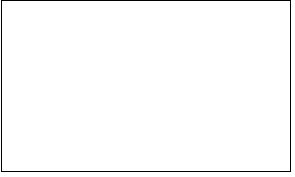
\includegraphics{figs/grabs.pdf}
% \end{graphicalabstract}

% Research highlights
\begin{highlights}
\item Research highlights item 1
\item Research highlights item 2
\item Research highlights item 3
\end{highlights}

% Keywords
% Each keyword is seperated by \sep
\begin{keywords}
quadrupole exciton \sep polariton \sep \WGM \sep \BEC
\end{keywords}


\maketitle













\printcredits

%% Loading bibliography style file
% \bibliographystyle{model1-num-names}
\bibliographystyle{cas-model2-names}

% Loading bibliography database
\bibliography{ref}


%\vskip3pt


\end{document}

